\documentclass[a4paper, oneside]{memoir}% Document class
\usepackage[a4paper]{geometry}			% Margins
\usepackage{lmodern}
\usepackage{graphicx}
\usepackage{float}
\usepackage{listings}
\usepackage[small,compact]{titlesec}	% No 'chapter' in chapter headings.
\graphicspath{{Media/}}					% Directory that holds images.

\titleformat{\chapter}[hang]
{\normalfont\Large\bfseries}{\thechapter}{1em}{\Large}
\titlespacing{\chapter}{0pt}{*0}{*1}

\titleformat{\chapter}{\Huge\bfseries}{\thechapter}{1em}{}
\titleformat{\section}{\LARGE\bfseries}{\thesection}{1em}{}
\titleformat{\subsection}{\Large\bfseries}{\thesubsection}{1em}{}
\titleformat{\subsubsection}{\normalsize\bfseries}{\thesubsubsection}{1em}{}


\author{
  Erik Sidelmann Jensen\\
  \texttt{ejens11@student.aau.dk}
  \and
  Lasse Vang Gravesen\\
  \texttt{lgrave11@student.aau.dk}
  \and
  Dennis Jakobsen\\
  \texttt{djakob11@student.aau.dk}  
}

\title{Web Intelligence - Recommender Miniproject}
\date{}

\begin{document}
	\clearpage\maketitle
	\thispagestyle{empty}
	
	\chapter{Recommender Miniproject}
	\section{Data Loading \& Manipulation}
	The structure used to contain the data being loaded is based on Dictionaries, specifically because we are provided with a movie and a user id and it makes sense to structure it like that.
	Actually loading is done by first loading the probe data and relevant information is put into a UserRating class that contains everything that is known about that rating(which movie and user).
	Then the training data is loaded, which is done the same way as the probe data.
	We only load movies that are represented in the probe dataset, and if also restrict it to very few files. 
	Then we manipulate the data such that we can run accuracy tests later, specifically we take the ratings from the training data that are represented in the probe data and add it to the representation and then we remove it from the training data. This is done because we want to see how accurately the rating can be estimated, and if the rating is already in the training data when the learning takes place we will not know how accurately it is actually guessing unknown ratings.
	
	The data being manipulated is not resaved because loading data is not a bottleneck for our purposes.
	
	\section{Learning}
	% ...
	There are two different recommender systems to use, being collaborative filtering and content-based filtering. For content-based filtering the content of an item is what you recommend based on. This information is however not present in the Netflix competition data. Only a movie-id, user-id and a rating is present in this data. Therefore a collaborative filtering recommender system is built.
	
	The next step in creating a CF recommender system, is to remove the movie and user means from the training data, in order to do some pre-processing for the algorithm, see Figure \ref{fig:obv}. We remove these means because we want to normalise the ratings to take into account the differences between peoples enthusiasm when rating. For example, one person could rate a movie with two star, where another person could rate the same movie four stars, but the meaning of the stars would be the same, because the first user has a tendency to rate low whereas the other user has a tendency to rate high.
	
	\begin{figure}[h]
		\centering
		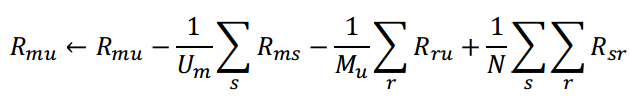
\includegraphics[scale=0.5]{obviousstructure}
		\caption{Removing the obvious structure from the ratings.}\label{fig:obv}
	\end{figure}
	
	\begin{description}
		\item $U_m$: total number of of observed ratings for movie $m$.
		\item $M_u$: total number of observed ratings for user $u$.
		\item $N$: total number of observed movie-user pairs.
	\end{description}
	
	We construct the movie feature A and the user feature B	by first filling it with random values between -0.5 and 0.5. Then we use the stochastic gradient descent algorithm to calculate A and B, see Figure \ref{fig:stocalg}. This algorithm iterates until the error reaches a local minimum, that is until the error becomes larger. We do not check the error for every iteration, but instead check it with some interval. It is not necessary to monitor this error for a minimum, since a predetermined amount of iterations can be used, for example 1 000 000, and just adjust this value until a minimum error has been reached.
	
	\begin{figure}[h]
			\centering
			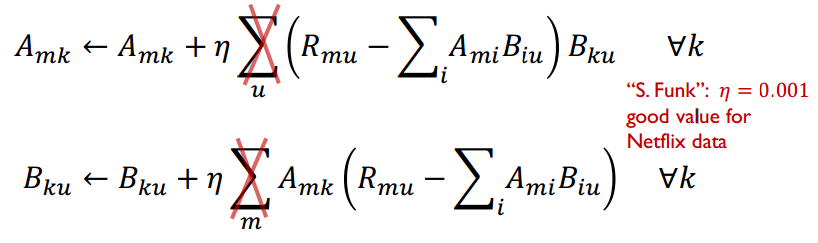
\includegraphics[scale=0.5]{sfunk}
			\caption{Stochastic gradient descent.}\label{fig:stocalg}
	\end{figure}
	
	\begin{description}
		\item $k$: Latent factors (between 10 and 50).
		\item $R_{mu}$: Rating for movie $m$ and user $u$.
		\item $\eta$: Learning rate.
	\end{description}
	
	At last, we add in the obvious structure from the pre-processing step again, and truncate the calculated rating to fit the Netflix rating scale. Every rating above five results in five, and all ratings below one results in one.
	
	Alternative algorithms could have been used such as user-based nearest neighbors CF (kNN) and item-based nearest neighbors CF (kNN). Although for these techniques there are issues with scalability when having millions of users and thousands of movies. Furthermore there are a possible problem of coverage where the kNN algorithm does not find enough neighbors and for example with user with preferences for niche products.
	
	Using this model-based algorithm matrix factorisation scales to larger data set. When recommending a movie to a user, only the learned model is used, which makes it much faster, although the model is re-trained or updated periodically.
	
	The model-based approach seems as the best choice for this kind of recommender system, although we did not manage to get useful results out of it.
	
	\section{Scoring}
	We evaluated the RMSE(Root-Mean-Square Error) for the probe data and the result ranged between 1.15 and 1.50, where it should roughly have been 0.90.
	
	$$RMSE = \sqrt{\frac{\Sigma_{i = 1}^{n} (\hat{r}_i - r_i)^2}{n}}$$
	
	For one subset of the overall dataset we did manage to get good results, specifically using midsized movie files and ~25 of them we could get an RMSE score of 0.90, though changing the latent factors seemed not to make much of a difference in the final result.

\end{document}
